% Free body diagram for the race-car problem.  Third of four composite figures
% for Lecture 7 (collocation), authored 2026-09-08.
%
% WHAT IT SHOWS, and where every number comes from.  The model is Eq. (7-car)
% in ../../optimization-private/lecture-notes/lectures/collocation.tex:
%
%     xdot = v,   vdot = u - R v^2,   m = 1
%     x(0) = 0, v(0) = 0;   x(t_f) = L, v(t_f) = 0;   -3 <= u <= 1
%
% which is Biegler's Example 8.5 (p. 229) -- the drag-free double integrator --
% with the quadratic drag term R v^2, the unit mass and the specific bounds
% added by Prof. Dowling.  So m = 1 makes vdot = u - R v^2 a force balance in
% which the numbers ARE accelerations, which is why u is labelled here as both.
%
% 🔴 THE ASYMMETRY OF THE BOUNDS IS THE POINT, and it is drawn to scale.  The
% lecture puts "strong brakes" under -3 and "modest engine" under 1; the
% feasible bar at the bottom of this figure is three times as long on the
% braking side as on the driving side, so the reader sees the asymmetry before
% reading the numbers.  Do not centre that bar for tidiness.
%
% GREYSCALE.  Two hues, and every arrow is distinguished three ways over:
%   * u   -- Okabe-Ito blue #0072B2 (L* = 46), SOLID rule, points FORWARD,
%            drawn below the axle line, directly labelled "u";
%   * Rv^2 -- Okabe-Ito orange #E69F00 (L* = 70.6), DENSELY DASHED, points
%            BACKWARD, drawn above the axle line, directly labelled "R v^2".
% dL* = 24.6, so they separate in print on hue alone as well.  README.md's
% "arrows are not series" rule is why both are labelled in place with the
% symbol they carry rather than by a legend.
%
% TIKZ LIBRARIES.  Base tikz plus >=stealth.  No calc, no patterns (the road
% hatching is drawn as explicit short strokes for exactly this reason), no
% decorations.pathreplacing.  Builds under both preambles.

\definecolor{cpblue}{HTML}{0072B2}
\definecolor{cporange}{HTML}{E69F00}

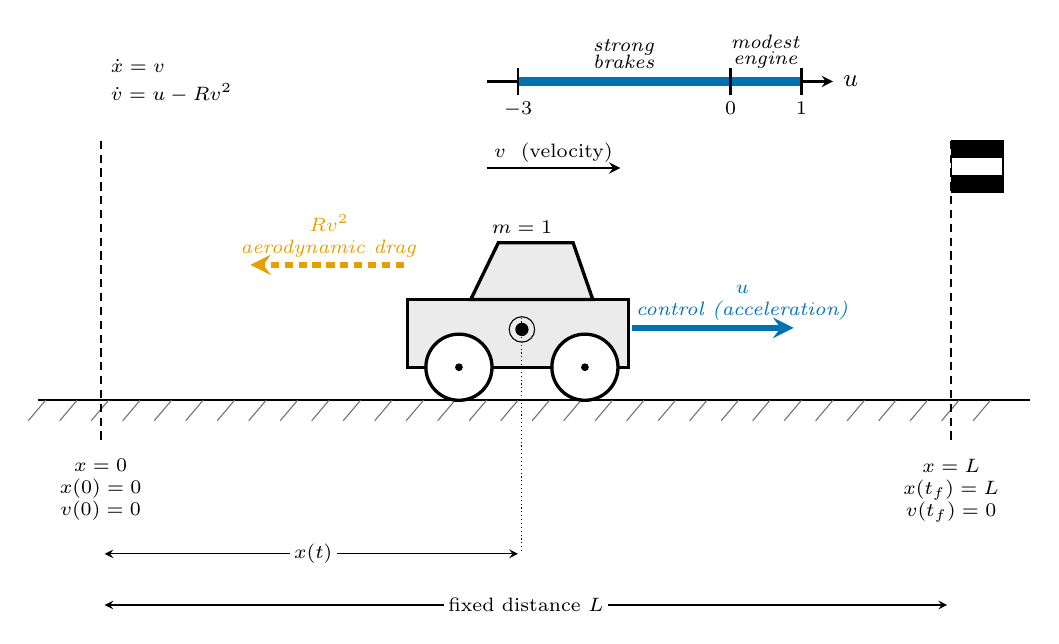
\begin{tikzpicture}[x=1cm, y=1cm, font=\small]

% ============================================================== the road
\draw[thick] (-0.2,0) -- (12.4,0);
\foreach \x in {-0.1,0.3,...,12.3}
  \draw[black!55] (\x,0) -- ++(-0.22,-0.26);

% ================================================== start and finish lines
\draw[thick, densely dashed] (0.6,-0.5) -- (0.6,3.3);
\node[below, align=center, font=\scriptsize] at (0.6,-0.62)
  {$x = 0$\\ $x(0)=0$\\ $v(0)=0$};

\draw[thick, densely dashed] (11.4,-0.5) -- (11.4,3.3);
\node[below, align=center, font=\scriptsize] at (11.4,-0.62)
  {$x = L$\\ $x(t_f)=L$\\ $v(t_f)=0$};
% Chequered flag, so the finish line reads as a finish line and not as just
% another dashed rule.
\foreach \k in {0,1,2} {
  \fill[black] (11.4+0.22*\k,3.3-0.22) rectangle ++(0.22,0.22);
  \fill[black] (11.4+0.22*\k,3.3-0.66) rectangle ++(0.22,0.22);
}
\draw (11.4,3.3-0.66) rectangle (11.4+0.66,3.3);

% ===================================================================== car
% Body, cabin and wheels.  Deliberately plain: this is a force diagram, not an
% illustration.
\draw[very thick, fill=black!8] (4.5,0.42) rectangle (7.3,1.28);
\draw[very thick, fill=black!8] (5.3,1.28) -- (5.65,2.0) -- (6.6,2.0)
                                -- (6.85,1.28) -- cycle;
\draw[very thick, fill=white] (5.15,0.42) circle (0.42);
\draw[very thick, fill=white] (6.75,0.42) circle (0.42);
\fill (5.15,0.42) circle (1.4pt);
\fill (6.75,0.42) circle (1.4pt);

% Centre of mass.  The mass label goes ABOVE THE ROOF, not beside the dot:
% inside the body it collides with the cabin, and the body is the one place in
% this drawing with no free space.
\fill (5.95,0.9) circle (2.4pt);
\draw (5.95,0.9) circle (4.6pt);
\node[above, font=\scriptsize, inner sep=2.5pt] at (5.95,2.02) {$m = 1$};

% ================================================== the two horizontal forces
% Control force u -- forward, SOLID, below the centre line.
\draw[cpblue, line width=2.2pt, ->, >=stealth] (7.35,0.92) -- (9.4,0.92);
\node[cpblue, above, align=center, font=\scriptsize, inner sep=2.5pt]
  at (8.75,0.92) {$u$\\ \emph{control (acceleration)}};

% Drag R v^2 -- backward, DASHED, above the centre line.
\draw[cporange, line width=2.2pt, densely dashed, ->, >=stealth]
  (4.45,1.72) -- (2.5,1.72);
\node[cporange, above, align=center, font=\scriptsize, inner sep=2.5pt]
  at (3.5,1.72) {$R v^2$\\ \emph{aerodynamic drag}};

% Velocity -- a kinematic quantity, not a force, so it is drawn THIN and BLACK
% well above the body where it cannot be mistaken for one of the two arrows.
\draw[thick, ->, >=stealth] (5.5,2.95) -- (7.2,2.95);
\node[above, font=\scriptsize, inner sep=2pt] at (6.35,2.95) {$v$ \ (velocity)};

% ==================================================== position and distance
\draw[<->, >=stealth] (0.65,-1.95) -- (5.9,-1.95);
\node[fill=white, inner sep=1.5pt, font=\scriptsize] at (3.3,-1.95)
  {$x(t)$};
\draw[densely dotted] (5.95,1.05) -- (5.95,-1.95);

\draw[<->, >=stealth] (0.65,-2.6) -- (11.35,-2.6);
\node[fill=white, inner sep=1.5pt, font=\scriptsize] at (6.0,-2.6)
  {fixed distance $L$};

% ============================================== the model, and the bounds
\node[align=left, font=\scriptsize, inner sep=3pt] at (1.5,4.05)
  {$\dot x = v$\\[2pt] $\dot v = u - R v^2$};

% Bound bar, DRAWN TO SCALE: -3 to 0 is three times the length of 0 to 1, so
% the asymmetry reads before the numbers do.  Do not centre it for tidiness.
% Origin of the bar at x = 8.6, one unit of u = 0.9 cm.
\draw[->, >=stealth, thick] (5.5,4.05) -- (9.9,4.05) node[right] {$u$};
\draw[cpblue, line width=3.2pt] (5.9,4.05) -- (9.5,4.05);
\foreach \u/\lab in {-3/{$-3$}, 0/{$0$}, 1/{$1$}} {
  \draw[thick] (8.6+0.9*\u,3.88) -- (8.6+0.9*\u,4.22);
  \node[below, font=\scriptsize, inner sep=2.5pt] at (8.6+0.9*\u,3.88) {\lab};
}
% Two lines each, so the two captions cannot run into one another -- they did,
% on one line, and printed as "strong brakesengine".
\node[above, align=center, font=\scriptsize, inner sep=2.5pt] at (7.25,4.12)
  {\emph{strong}\\[-2pt] \emph{brakes}};
\node[above, align=center, font=\scriptsize, inner sep=2.5pt] at (9.05,4.12)
  {\emph{modest}\\[-2pt] \emph{engine}};

\end{tikzpicture}
